\documentclass[12pt]{article}
\usepackage[utf8]{vietnam}
\usepackage[vietnamese,english]{babel}
\usepackage{tocloft}
\renewcommand{\cftsecleader}{\cftdotfill{\cftdotsep}} % for sections, if you really want! (It is default in report and book class (So you may not need it).
\usepackage{float}
\usepackage{graphicx}
\usepackage{subfig}
\usepackage[dvipsnames]{xcolor}
\usepackage[colorlinks=true,linkcolor=blue,urlcolor=red,citecolor=magenta]{hyperref}
\usepackage{amsmath,amssymb,amsthm}
\allowdisplaybreaks
\usepackage[splitrule]{footmisc} %% The splitrule option draws a full width rule above the continued part of the footnote as a visual cue to readers.
\numberwithin{equation}{section}
\newtheorem{assumption}{Assumption}[section]
\newtheorem{lemma}{Lemma}[section]
\newtheorem{corollary}{Corollary}[section]
\newtheorem{definition}{Definition}[section]
\newtheorem{proposition}{Proposition}[section]
\newtheorem{theorem}{Theorem}[section]
\newtheorem{notation}{Notation}[section]
\newtheorem{remark}{Remark}[section]
\newtheorem{example}{Example}[section]
\newtheorem{ques}{Question}[section]
\newtheorem{problem}{Problem}[section]
\newtheorem{conjecture}{Conjecture}[section]
\usepackage[left=0.5in,right=0.5in,top=1.5cm,bottom=1.5cm]{geometry}
\usepackage{fancyhdr}
\pagestyle{fancy}
\fancyhf{}
\addtolength{\headheight}{0pt} % obsolete
\lhead{\small \textsc{Sect.} ~\thesection}
\rhead{\small \nouppercase{\leftmark}} % \nouppercase !
\renewcommand{\sectionmark}[1]{\markboth{#1}{}}
\cfoot{\thepage}

\title{Psychological Manipulation}
\author{Nguyễn Quản Bá Hồng}
\date{\small\textsf{Version: \today}}

\begin{document}
\maketitle
\setcounter{secnumdepth}{6}
\setcounter{tocdepth}{6}

%------------------------------------------------------------------------------%

\begin{abstract}
    What ``\textit{psychological manipulation}'' is, why and how to detect and conquer it.\footnote{Download the latest version at the following \textsc{url}: \url{https://github.com/NQBH/miscellaneous/blob/master/blog/psychological_manipulation/NQBH_psychological_manipulation.pdf} with different size options: [\href{https://github.com/NQBH/miscellaneous/blob/master/blog/psychological_manipulation/NQBH_psychological_manipulation_size_10pt.pdf}{10pt}][\href{https://github.com/NQBH/miscellaneous/blob/master/blog/psychological_manipulation/NQBH_psychological_manipulation_size_11pt.pdf}{11pt}][\href{https://github.com/NQBH/miscellaneous/blob/master/blog/psychological_manipulation/NQBH_psychological_manipulation_size_12pt.pdf}{12pt}].}
\end{abstract}

\noindent
\textbf{Keywords.} [\textit{en}-vi]
\begin{itemize}
    \setlength\itemsep{0em}
    \item \textit{Psychological manipulation} - Thao túng tâm lý
    \item \textit{Psychological abuse}\texttt{/}\textit{violence, emotional}\texttt{/}\textit{mental abuse} - Lạm dụng\texttt{/}bạo lực tâm lý\texttt{/}cảm xúc
    \item \textit{Breaking point} - Điểm gãy\texttt{/}vỡ\texttt{/}nguy kịch
    \item \textit{Social isolation} - Cô lập xã hội
    \item \textit{Anxiety disorder} - Rối loạn lo âu
    \item \textit{Depression} - Trầm cảm
\end{itemize}

\tableofcontents

\section{\texttt{{\color{RubineRed}\#include} ``basic terminologies''}}
I have not read yet, and unintended to, all the heavy references mentioned in this section, but they seem necessary to be included for the sake of completeness.

\begin{definition}[Psychological manipulation \cite{Psychological Wiki/Psychological manipulation,Wikipedia/Pyschological manipulation}]
    \emph{Psychological manipulation} is a type of \href{https://psychology.wikia.org/wiki/Social_influence}{social influence} that aims to change the \href{https://en.wikipedia.org/wiki/Perception}{perception} or behavior of others through underhanded, \href{https://en.wikipedia.org/wiki/Deceptive}{deceptive}, or even \href{https://psychology.wikia.org/wiki/Abuse}{abusive} tactics (\cite{Braiker2004}). By advancing only the interests of the manipulator, often at the other's expense, such methods could be considered exploitative, abusive, devious, and deceptive.
\end{definition}

\begin{definition}[Psychological abuse\texttt{/}violence, emotional\texttt{/}mental abuse \cite{Psychology Wiki/Abusive relationship,Wikipedia/Psychological abuse}]
    \emph{Psychological abuse}, often called \emph{emotional abuse}, is a form of \href{https://en.wikipedia.org/wiki/Abuse}{abuse}, characterized by a person subjecting or exposing another person to behavior that may result in \href{https://en.wikipedia.org/wiki/Psychological_trauma}{psychological trauma}, including \href{https://en.wikipedia.org/wiki/Anxiety_disorder}{anxiety}, \href{https://en.wikipedia.org/wiki/Chronic_depression}{chronic depression}, or \href{https://en.wikipedia.org/wiki/Post-traumatic_stress_disorder}{post-traumatic stress disorder} (\cite{Dutton1994,Dutton_Goodman_Bennett2000,Thompson_Kaplan1996}). It is often associated with situations of \href{https://en.wikipedia.org/wiki/Abusive_power_and_control}{power imbalance in abusive relationships}, and may include \href{https://en.wikipedia.org/wiki/Bullying}{bullying}, \href{https://en.wikipedia.org/wiki/Gaslighting}{gaslighting}, and \href{https://en.wikipedia.org/wiki/Workplace_bullying}{abuse in the workplace} (\cite{Dutton_Goodman_Bennett2000,Thompson_Kaplan1996}). It also may be perpetrated by persons conducting \href{https://en.wikipedia.org/wiki/Torture}{torture}, other \href{https://en.wikipedia.org/wiki/Violence}{violence}, acute or prolonged \href{https://en.wikipedia.org/wiki/Human_rights_abuse}{human rights abuse}, particularly without legal redress such as \href{https://en.wikipedia.org/wiki/Detention_without_trial}{detention without trial}, \href{https://en.wikipedia.org/wiki/False_accusation}{false accusations}, false convictions and extreme \href{https://en.wikipedia.org/wiki/Defamation}{defamation} such as where perpetrated by state and media. 
\end{definition}

\begin{definition}[Breaking point (psychology) \cite{Wikepedia/Breaking point (psychology)}]
    In human psychology, the \emph{breaking point} is a moment of \href{https://en.wikipedia.org/wiki/Stress_(medicine)}{stress} in which a person breaks down or a situation becomes critical.
\end{definition}
``The intensity of environmental stress necessary to bring this about varies from individual to individual.''

\begin{definition}[Social isolation \cite{Wikipedia/Social isolation}]
    \emph{Social isolation} is a state of complete or near-complete lack of contact between an individual and \href{https://en.wikipedia.org/wiki/Society}{society}. It differs from \href{https://en.wikipedia.org/wiki/Loneliness}{loneliness}, which reflects temporary and involuntary lack of contact with other humans in the world. Social isolation can be an issue for individuals of any age, though symptoms may differ by age group.
\end{definition}
``Social isolation has similar characteristics in both temporary instances and for those with a historical lifelong isolation cycle. All types of social isolation can include staying home for lengthy periods of time, having no communication with family, acquaintances or friends, and\texttt{/}or willfully avoiding any contact with other humans when those opportunities do arise.''

See also, e.g. \cite{NASEM2020,NhuTrang2020}.

\begin{definition}[Anxiety disorder \cite{Wikipedia/Anxiety disorder}]
    \emph{Anxiety disorders} are a group of \href{https://en.wikipedia.org/wiki/Mental_disorder}{mental disorders} characterized by significant feelings of \href{https://en.wikipedia.org/wiki/Anxiety_(mood)}{anxiety} and \href{https://en.wikipedia.org/wiki/Fear}{fear}. Anxiety is a worry about future events, while fear is a reaction to current events. These feelings may cause physical symptoms, such as increased heart rate and shakiness. There are several anxiety disorders, including \href{https://en.wikipedia.org/wiki/Generalized_anxiety_disorder}{generalized anxiety disorder}, \href{https://en.wikipedia.org/wiki/Specific_phobia}{specific phobia}, \href{https://en.wikipedia.org/wiki/Social_anxiety_disorder}{social anxiety disorder}, \href{https://en.wikipedia.org/wiki/Separation_anxiety_disorder}{separation anxiety disorder}, \href{https://en.wikipedia.org/wiki/Agoraphobia}{agoraphobia}, \href{https://en.wikipedia.org/wiki/Panic_disorder}{panic disorder}, and \href{https://en.wikipedia.org/wiki/Selective_mutism}{selective mutism}. The disorder differs by what results in the symptoms. An individual may have more than one anxiety disorder.
\end{definition}
See the main reference: \cite{APA2013}.

\begin{definition}[Depression (mood) \cite{Wikipedia/Depression (mood)}]
    \emph{Depression} is a state of low \href{https://en.wikipedia.org/wiki/Mood_(psychology)}{mood} and aversion to activity. It can affect a person's thoughts, behavior, motivation, \href{https://en.wikipedia.org/wiki/Feeling}{feelings}, and \href{https://en.wikipedia.org/wiki/Subjective_well-being}{sense of well-being}. The core symptom of depression is said to be \href{https://en.wikipedia.org/wiki/Anhedonia}{anhedonia}, which refers to loss of interest or a loss of feeling of pleasure in certain activities that usually bring joy to people. Depressed mood is a symptom of some \href{https://en.wikipedia.org/wiki/Mood_disorders}{mood disorders} such as \href{https://en.wikipedia.org/wiki/Major_depressive_disorder}{major depressive disorder} or \href{https://en.wikipedia.org/wiki/Dysthymia}{dysthymia}; it is a normal temporary reaction to life events, such as the loss of a loved one; and it is also a symptom of some physical diseases and a \href{https://en.wikipedia.org/wiki/Side_effect}{side effect} of some drugs and medical treatments. It may feature sadness, difficulty in thinking and concentration and a significant increase or decrease in appetite and time spent sleeping. People experiencing depression may have feelings of dejection, hopelessness and, sometimes, suicidal thoughts. It can either be short term or long term. 
\end{definition}
See also, not e.g. as usual but especially this time, \cite{Solomon2015}.

\begin{verbatim}
    // * * * * * * * * * * * * * * * * * * * * * * * * * * * * * * * * * * * * * //
\end{verbatim}

\section{\texttt{{\color{cyan}\textit{int}} {\color{YellowGreen} main} ({\color{cyan}\textit{int}} argc, {\color{cyan}\textit{char}} *argv[]) \{}}

\fbox{\textbf{1}} \textit{Just another winter's day}$\ldots$

\begin{figure}[H]
    \centering
    
\includegraphics[width=0.75\textwidth]{Berlin_winter2020}
    \caption{Winter 2020, Berlin, Germany.}
    \label{fig1}
\end{figure}
Light precipitation (rain $+$ snow) outside the window (see Fig. \ref{fig1})$\ldots$ The room is so quiet that I can even hear my own heartbeat when I lay down: So annoying (see Fig. \ref{fig2})$\ldots$

\begin{figure}[h]
    \centering
    
\includegraphics[width=0.75\textwidth]{Arima_Kousei_you_are_in_my_way}
    \caption{Arima Kousei's emotional explosion when performing piano with Nagi, Episode 18: \textit{Hearts Come Together}, \textit{Your Lie in April} (2014--2015).}
    \label{fig2}
\end{figure}

\begin{quotation}
    ``\textit{I can't concentrate. I can still hear the sound of the piano. It's in my way. You're in my way, so$\ldots$ Get out of here!}'' - Arima Kousei, \textit{Your Lie in April} (2014--2015).
\end{quotation}

I always have this kind of weird feeling\footnote{An indication of bad writing?} when I try to write something and connect all, or as many as possible, the ideas in my flow of thoughts together, you know? This even does not sound right to me because the question is: \textit{How the hell you can organize and \href{https://en.wikipedia.org/wiki/Connect_the_dots}{connect the dots} when that flow in your head is a real shitty mess?}

In such a situation, as usual, a bad writing habit [no chronological order, switch randomly between English and Vietnamese\footnote{\textit{If the real purpose is to express your thoughts\texttt{/}ideas\texttt{/}emotions, why does it matter to write under a lot of unnecessary\texttt{/}redundant chains\texttt{/}constraints\texttt{/}criteria?}}, etc.] can be partially accepted and invoked as an unavoidable replacement to a ``standard'' one: \textit{Just let it all out naturally$\ldots$}

\begin{verbatim}
    // * * * * * * * * * * * * * * * * * * * * * * * * * * * * * * * * * * * * * //
\end{verbatim}

\noindent
\fbox{\textbf{2}} Đã mấy tháng nay, mình thường cố ý đi làm trễ khoảng 1 tiếng, để đợi những người khác đến chỗ làm gần đủ hết, vì mình chỉ muốn tránh thủ tục chào hỏi xởi lởi\texttt{/}xã giao ``khích lệ tinh thần'' phiền phức mỗi buổi sáng. Mình đánh hơi thấy mùi fake và bắt đầu trở lên im lặng như một năm về trước. Mình cũng dần dần hiểu được phần nào ý nghĩa của từ ``guồng'' mà các anh lớn hơn với thằng bạn mình hay nhắc tới: Mọi thứ [công việc + cuộc sống cá nhân] bắt đầu lặp đi lặp lại một cách đơn điệu (monotonously), màu sắc cứ dần dần mà phai nhạt ngày qua ngày$\ldots$

À xém chút quên ngữ cảnh, khi những dòng này được viết, mình đã nếm trải 10 tháng đầu tiên của hành trình làm nghiên cứu sinh ở Đức\footnote{Usually called ``PhD'' in general and ``Doktorand'' in German.} bên Applied Math, cụ thể là về Tối Ưu Hình Dáng\footnote{Dịch thuật ngữ chuyên ngành toán ra tiếng việt thường mang lại cảm giác củ chuối như vậy! Sad$\ldots$} (\href{https://en.wikipedia.org/wiki/Shape_optimization}{Shape Optimization}) cho ống dẫn khí của động cơ đốt trong. Khi mới bắt đầu làm thì mình thấy thích topic này lắm, nhưng đến giữa chừng thì lại bắt đầu chán. \textit{Là do mình hay công việc nghiên cứu nó vốn tẻ nhạt như vậy?}$\ldots$

\begin{verbatim}
    // * * * * * * * * * * * * * * * * * * * * * * * * * * * * * * * * * * * * * //
\end{verbatim}

\noindent
\fbox{\textbf{3}} Vào một ngày đông nào đó (vì bữa đó quá đỗi bình thường nên mình chả thèm\texttt{/}thể nhớ chính xác là ngày nào) mình lại đạp xe đến chỗ làm, cố gắng tránh né ánh mắt của mọi người. Đến trưa thì đợi ông thầy phụ của mình đi rủ họ ăn chung với nhau, rồi mình lại xách hộp cơm tự nấu đem theo ra khỏi tòa nhà, đến công viên đối diện để ngồi ăn giữa trời tuyết: \textit{lủi thủi} và \textit{cô độc}. Vừa ăn trưa mình vừa ngắm chim (ở Berlin chim bồ câu đâu ra cả nùi nùi và đặc biệt là tụi chim này rất dạng, chắc đất chốn đây hẳn là lành lắm!). Một lát sau mình lại lết lên phòng làm việc. \textit{Nặng nề} và \textit{ủ dột}, mình vẫn phải tiếp tục làm những tasks được giao nhưng không hề cảm thấy thích như mọi khi mình được tự ý làm những thứ mình tự chế\texttt{/}bày ra nữa. Haizz$\ldots$ Cố làm vậy, rồi từ từ cũng sẽ hết ngày, lại đi về, nấu cơm ăn, xem YouTube đến khi mỏi mắt, rồi ngủ, rồi ngày sau lại lặp lại y như thế: \textit{Ôi cái guồng này nó làm mình chán phát điên mất} - mình vừa làm vừa nghĩ vậy$\ldots$

Đợi đến tầm xế chiều, thì cô bạn Maroc ngồi đối diện lưng-lưng (not mặt-mặt) với mình moi ra một hộp Chocolate để tặng mình. Hề cái là cô này phải đợi anh bạn người Đức chung phòng đi lấy\texttt{/}nhả nước gì đấy thì cổ mới có dịp để tặng riêng cho mình (phòng mình là phòng toàn PhDs duy nhất của cả nhóm, gồm 3 đứa mình). Tỏ tình? Nah, nhìn lại cái thân hình đang ngày càng trì trệ\footnote{Ironically, I am currently working on Shape Optimization but my body shape gets far and far away from ``optimal''.} mấy tháng qua của mày đi. Đùa chứ bản nói vì mình đã giúp bản rất nhiều thủ tục giấy tờ - mà mình đã phải vật lộn rất nhiều trong mấy tháng đầu nhờ đợt dịch - khi mới tới nên bản biết hơn (mình đổi từ ``cổ'' sang ``bản'' vì mình để ý tên email riêng của cổ: à, thì ra cô này bằng tuổi mình). Bản nói bản biết ơn mình và ông thầy phụ của mình lắm, trong mắt cô bạn mới tới thì đây là 2 người tử tế giúp đỡ bản nhiều nhất trong nhóm$\ldots$

\textit{Ồ, thì ra vẫn có người trong nhóm xem mình là người tốt\texttt{/}tử tế à?} Thật tình thì lúc mình giúp cô bạn thì mình chả nghĩ gì nhiều, giúp thì giúp thôi. Mình là kiểu người ngu dốt kiểu vậy. À không, còn tệ hơn nhiều cơ: \textit{a giver}\footnote{\href{https://www.youtube.com/watch?v=YyXRYgjQXX0}{Are you a giver or a taker? | Adam Grant}, TED.}. Việc mình trở thành 1 giver chắc là do ảnh hưởng từ mẹ mình. Hồi nhỏ mẹ mình hay dạy là con cứ tốt với mọi người xung quanh thì họ sẽ tốt lại với con thôi, chứ đừng cứ sống ích kỷ rồi không ai chơi với con hết, đại loại vậy. Đó cũng là bài học đối nhân xử thế đầu tiên của mình và ảnh hưởng đến tính cách mình rất nhiều$\ldots$

Nghe cô bạn cảm ơn, mình nhìn hộp Chocolate, một chút vui thoáng qua nhưng cũng chợp tắt thật nhanh. Mình không cho phép mình vui lâu hơn vì chắc gì đó là những lời thật lòng, hay \textit{chẳng qua chỉ là xã giao với nhau để được giúp nhiều hơn mà thôi?} Vì mình hiểu rằng bất kể mình có tốt bụng và tử tế cỡ nào đi chăng nữa, cô bạn này sau một thời gian nữa sẽ ghét và khinh mình vì những lời xuyên tạc từ những người khác trong những bữa ăn trưa tưởng chừng như thân thiện giữa các đồng nghiệp với nhau đó mà thôi$\ldots$

Một lúc sau thì anh bạn Đức về phòng. Anh này hiện đang chí mí cuối năm cuối PhD và đang bức tốc để chuẩn bị về đích\texttt{/}lên đỉnh Olympia, à nhầm, bảo vệ. Mình ngỏ ý chia 50--50 với ảnh, để cho không khí trong phòng 3 đứa mình đỡ căng thẳng. Anh từ chối thẳng, yêu cầu mình để anh ấy yên, anh ta không cần bất cứ thứ gì từ mình. Uầy, vô tình chuốc thêm căng thẳng rồi. Ngu người thật. Đành ăn một mình vậy. Bụng mập càng thêm mập$\ldots$

Cô bạn nói mình lần sau sẽ mua loại ngon hơn, lần này thì chỉ còn loại đó. Có vẻ thật lòng - mình nghĩ. Xem ra mình còn chút hy vọng xót lại vào humanity trong mối quan hệ giữa người với người. Mà nếu cô bạn canh để tặng quà Giáng sinh thì bữa đó là ngày 18 tháng 12, ngày đi làm cuối cùng của năm 2020, giờ mình mới có manh mối để nhớ ra ngày đó. Mùa nghỉ đông đầu tiên kéo dài hơn 40 ngày cuối cùng cũng bắt đầu\ldots

\begin{verbatim}
    // * * * * * * * * * * * * * * * * * * * * * * * * * * * * * * * * * * * * * //
\end{verbatim}

\noindent
\fbox{\textbf{4}} Khoảng thời gian nghỉ đông này rất quý giá để mình đầu tư vào work-life balance lại, bằng cách$\ldots$ làm việc nhiều hơn và đặc biệt là chỉ làm những thứ mình muốn, chứ không phải những tasks nhàm chán, đôi khi ngu xuẩn, mà ông thầy phụ mình cứ thảy cho suốt mấy tháng qua. Đó là cũng là khoảng thời gian yên tĩnh để mình có thể suy nghĩ về những chuyện đã xảy ra trong những tháng qua. Có vài chuyện mình không tài nào hiểu nổi, đương nhiên vẫn là những câu chuyện muôn thuở về mối quan hệ giữa con người với con người. Mình mà lị: \textit{The Trouble Boy}!!$\ldots$ Đại loại là, từ lúc mới đến Berlin tới giờ, bất kể mình giúp đỡ những người khác mỗi khi họ cần, họ đều cư xử toxic ngược lại, thậm chí có anh postDoc còn verbally bully mình. Thế mà mình cứ ảo\texttt{/}hoang tưởng là họ hoan nghênh mình tới để làm việc, trao đổi kiến thức và cống hiến cơ đấy, nhưng thì ra suất Marie--Curie này không dễ ăn\texttt{/}handled như mình vẫn tưởng bở. Môi trường học thuật mà thằng ngu này! Mình lại suy nghĩ quá đơn giản rồi. Chán cái đầu nông cạn\texttt{/}ngây thơ (naive) của mình thật! Thôi cứ đành ngậm họng lại, tránh tiếp xúc với mọi người (đương nhiên là ngoại trừ boss bự với boss nhỏ, ngu thì ngu chứ chưa muốn bị đuổi!) để khỏi bị bắt nạt, và giữ năng lượng để tập trung làm việc vậy$\ldots$ Còn 2 năm mấy, 3 năm nữa cơ mà! Đừng có kiểu mới nhập Viện chưa bao lâu mà đã gục\texttt{/}tịt ngòi chứ!$\ldots$

Ấy vậy mà, mặc dù đã tập trung làm việc miệt mài, tinh thần và cảm xúc mình vẫn bị kéo xuống liên tục, và các mối quan hệ với đồng nghiệp cứ thế càng ngày càng tệ: \textit{Thà không có thì tốt biết mấy!} - Mình chợt nghĩ. Cứ thế này thì mình sẽ bị vắt kiệt (drained out\texttt{/}\href{https://en.wikipedia.org/wiki/Occupational_burnout}{occupational burnout}) mất. Hóa ra hy vọng, niềm hân hoang, etc. chỉ là những thứ cảm xúc vô nghĩa mình tự tạo ra, để tự huyễn hoặc, và làm tiền đề cho sự chán chường nặng nề và thất vọng tột độ mà thôi$\ldots$

Được cái là ông thầy phụ (co-supervisor) của mình rất có tâm. Ổng giúp mình rất nhiều khi mình mới tới Berlin, từ cả nhà cửa, giấy tờ thủ tục, đến hầu hết tất cả các khía cạnh trong công việc. Nhận ra mình đang có dấu hiệu xuống tinh thần, ổng đôn đốc mình làm việc nề nếp, khoa học hơn, giao nhiều tasks hơn, và rồi cứ 4 giờ chiều mỗi ngày mình sẽ đến tận phòng để gặp và báo cáo ổng theo mệnh lệnh ở Thư viện chung, trước mặt của các nữ sinh viên đang học Master của nhóm. Thật tình thì đa số mấy tasks ổng giao mấy tháng gần đây có phần ngô nghê và vớ vẩn thiệt. \textit{Hay lúc nào cũng nhảm vậy nhỉ? Hay do mình đã tiến bộ mà không tự nhận thức được?} Không phải chảnh, đơn giản vì mình là người trực tiếp upgrade software, line-by-line, nên mình hiểu rõ nhiều cái technicals mất dạy mà phải tốn có khi cả tháng mới vượt qua được, nên nhiều cái ổng không biết mà chỉ bậy\texttt{/}bừa\texttt{/}xàm cũng không phải là điều quá ngạc nhiên. Mình là người kiểu vậy: Không quan trọng supervisor khủng (vì họ chỉ tổ bận mà thôi), chỉ cần supervisor có tâm là được. Tình cảm thầy trò vẫn quan trọng hơn là những danh tiếng hào nhoáng (reputation) mà mình chỉ hưởng xoáy chứ không phải có được nhờ chính thực lực của mình.

Tasks ngu thì ngu nhưng kệ vậy, miễn ổng tốt với mình là được rồi, cứ làm nhiệm vụ được giao vậy. Rồi sẽ ổn cả thôi, dù ảm đạm và cô độc đến cỡ nào đi nữa$\ldots$

\begin{verbatim}
    // * * * * * * * * * * * * * * * * * * * * * * * * * * * * * * * * * * * * * //
\end{verbatim}

\noindent
\fbox{\textbf{5}} Mình chợt nhớ lại 10 tháng trước. \textit{Mình làm ở đây mới có 10 tháng thôi mà đã thay đổi nhiều vậy cơ á?} 10 tháng trước, mình lao vào giữa vùng dịch, để làm lại từ đầu lần nữa. Quyết liệt và dữ dội, tưởng chừng không có gì cản trở được mình nữa, thì mình lại bắt đầu có dấu hiệu gục hệt như một năm trước lúc mình học Master về Pure\footnote{``Pure'', not ``poor''. But, actually, they sound similar. And that is exactly the reason why I have switched from Pure Math to Applied Math.} Math ở Pháp. Thật tự đáng hổ thẹn và thất vọng$\ldots$

Khoảng thời gian nghỉ đông tĩnh lặng và lạnh lẽo giúp mình có thể tập trung suy nghĩ sâu hơn, về nhiều thứ cực kỳ mâu thuẫn đã và đang diễn ra khiến mình thật sự bối rối và bắt đầu nghi ngờ. Điều này làm mình chợt nhớ lại cuốn sách \cite{Bancroft2003} về ``\textit{Kẻ thao túng tâm lý\texttt{/}bạo hành tinh thần}'', mà mình biết tới nhờ một lần đọc một psychology post về ``\textit{Kẻ bạo hành âm thầm}''. Well, thực tình mà nói đây là một cuốn sách về bạo hành gia đình, cả bạo hành thể chất lẫn bạo hành tâm lý nhưng chú trọng đặc biệt về bạo hành tâm lý, cụ thể là tác động từ người chồng gia trưởng lên người vợ lẫn những đứa con đáng thương của ông ta. \textit{Daijoubu desu!} Mình vẫn còn con nít mà, nên vẫn có thể áp dụng vế sau lên chính trường hợp của mình được!

\textit{Một luồng những suy nghĩ, câu hỏi tự vấn từ sâu trong nội tâm bắt đầu tuôn trào}\footnote{Actually, I have been seriously overthinking about my overthinking problem all the time!$\ldots$ \textit{Wait, should I overthink about that also?!!}}$\ldots$

\begin{verbatim}
    // * * * * * * * * * * * * * * * * * * * * * * * * * * * * * * * * * * * * * //
\end{verbatim}

\noindent
\fbox{\textbf{6}} \textit{Another flow of thoughts}$\ldots$
\begin{itemize}
    \setlength\itemsep{0em}
    \item \textit{Why did almost all of my colleagues treat me so toxic like that despite the fact that I have helped them several times whenever they asked me for my hand. Don't they understand what the term ``grateful'' really means?}
    \item \textit{Why does a good person like me have to suffer all these toxic behaviors in lab-environment and even social isolation?}
    \item \textit{Is this world designed for good\texttt{/}kind people?}
    \item \textit{Does there exist a place on this Earth for all human beings with full of purely good intentions to live and work?}
    
    In a moment, it seems to me that there is no place for a person with low \href{https://en.wikipedia.org/wiki/Emotional_intelligence}{Emotional Intelligence} (EQ) and very low \href{https://en.wikipedia.org/wiki/Social_intelligence}{Social Intelligence} (SI) but \href{https://hsperson.com/}{Highly Sensitive} (HSP) like me in this cruel world.    
    \item \textit{Why do I have to avoid all these people and develop psychological problems, especially \href{https://en.wikipedia.org/wiki/Impostor_syndrome}{imposter syndrome}\footnote{The \#1 mental illness in academic\texttt{/}lab environment?}?} I have conducted a lot of tasks, even much more than my predecessors, then \textit{why do I have to keep suffering?}
    \item \textit{Why were I called ``The Lucky Guy''? Why does hardly anybody give a minimum level of respect to me even when I have been conducting such a huge amount of work? Is it because my skin is too yellow to be considered white enough?}
    \item \textit{Why do I have to do these stupid\texttt{/}bullshit tasks and report daily to my co-supervisor. And especially, whenever I refused to do such an unnecessary\texttt{/}redundant task, he started to be wildly angry immediately?} But he is a truthfully good, kind, honest, and enthusiastic co-supervisor, because he has helped me a lot through these tough times in this strange year.
\end{itemize}
I really do not understand: \textit{absolutely confused} and \textit{overwhelmed}$\ldots$

\textit{Tại sao mình có cảm giác bị đâm lén sau lưng liên tục nhưng không biết chính xác là ai cả? Tại sao ai cũng đối xử mình như thứ rác rưởi mặc dù mình giúp họ khá nhiều? Tại sao mình cảm giác bản thân không đủ tốt và làm việc chưa đủ cần cù trong khi mình đã làm được những điều mà những người tiền nhiệm ở vị trí của mình chưa từng làm được: ví dụ nâng cấp phần mềm được phát triển và sử dụng suốt 10 năm trong vòng chưa tới 10 tháng?}

Yeah, everything is so weird, very weird, super weird. This kind of feeling is exactly like there is an invisible ``Black Hole of Truth'' somewhere behind your back. You can feel its existence as a blur, but you cannot see it or touch it directly. So annoying$\ldots$ Very tired$\ldots$ Completely exhausted$\ldots$

- \textit{Can you figure out the reason why I hate such a ``Black Hole'' that much?}

- Is it because that hole is black?

- No, you racist fuck! Because$\ldots$ Like the way every matter, e.g. light (`photon') is rapidly sucked towards the `singularity' at the center of a real \href{https://en.wikipedia.org/wiki/Black_hole}{Black Hole}, all truths are also sucked towards this ``Truth Destroyer'' and then demolished/consumed by it.

\begin{verbatim}
    // * * * * * * * * * * * * * * * * * * * * * * * * * * * * * * * * * * * * * //
\end{verbatim}

\noindent
\fbox{\textbf{7}} \textit{Có phải mình đang cố đổ lỗi lên mọi người xung quanh để chối bỏ mọi chuyện tệ hại là lỗi của mình không?}

- Không hề.

- Xì\texttt{/}hừm\texttt{/}hứ\texttt{/}etc., thằng nhãi ranh đó lại thế, chả bao giờ biết tự nhận\texttt{/}chịu trách nhiệm (take the responsibility), chỉ biết đổ lỗi lên đầu người khác. Xem ra việc làm nghiên cứu sinh tưởng chừng sẽ giúp nó trưởng thành, chín chắn hơn phần nào nhưng giờ nó lại thế, vẫn thế, có khi còn tệ hơn! Đảm bảo nó sẽ mãi là đứa con nít không bao giờ lớn nổi.

- Ừm, có khi nói vậy cũng đúng phần nào$\ldots$

Tới đây thì bạn cần hiểu một điều rằng: \textit{khi bạn tự thấu hiểu chính bản thân từ bên trong, thì mọi lời phán xét\texttt{/}đàm tiếu bên ngoài không còn quan trọng nữa}$\ldots$

Mình không thể nào nói là mình không quan tâm (I do not care!) tới những lời phán xét như vậy, bởi vì thực sự là mình có quan tâm. Mình quan tâm là vì mình muốn bảo vệ sự thật (lại một hành động ngu xuẩn nữa trong chuỗi dài những hành động ngu xuẩn: scientist wannabe, huh?). Và một trong những bước cốt lõi để bảo vệ sự thật đó là phát hiện những lời giả dối\texttt{/}đàm tiếu\texttt{/}vu khống (Lie Detector) và điều chỉnh những lời phát xét bị biến dạng (distorted judgments) do tác dụng của chính cái ``Black Hole of Truth'' gây ra$\ldots$

\textit{Bạn biết vì sao nhiều người thích phán xét thế không?} Đó là vì việc phán xét rất dễ: không cần phải suy nghĩ\texttt{/}động não nhiều, không cần tốn quá nhiều sức, chỉ cần hướng thẳng tới việc công kích\texttt{/}đả thương người khác là bất cứ ngôn từ nào phát ra từ miệng một người tự nhiên\texttt{/}tự động\texttt{/}mặc định trở thành lời phát xét tiêu cực (đôi khi chết người) ngay lập tức. \textit{Thế thì nghe tiêu cực nhỉ? Nhưng nếu bản chất là tiêu cực vậy thì tại sao còn những người muốn làm điều như vậy?} Nhiều là đằng khác! Đó là vì: phán xét tuy rất dễ nhưng đem lại rất nhiều cảm giác sảng khoái cho ``người thẩm phán'': cảm giác tha hồ nếm trải quyền lực\texttt{/}sự thống trị  lấn át lên trên nạn nhân để thỏa mãn cái tôi mà không cần tốn nhiều sức lực. Trái lại, việc bình tĩnh suy nghĩ một cách thấu đáo để thực sự hiểu một vấn đề lại khó hơn rất nhiều: đòi hỏi đầu tư nhiều thời gian và công sức hơn, và đặc biệt là những kinh nghiệm tích lũy mà thông thường chỉ những người từng trải và\texttt{/}hoặc đủ khôn ngoan\texttt{/}sáng suốt mới có được. Mặc dù cần đầu tư nhiều như vậy, nhưng điều nực cười là việc thấu cảm (also thấu hiểu, cảm thông) thường không nhận được bất kỳ sự ủng hộ nào từ số đông do ảnh hưởng của tư tưởng bầy đàn\texttt{/}hiệu ứng đám đông\footnote{Điều này là đối tượng nghiên cứu chính của nhánh chuyên ngành Tâm lý học đám đông của Tâm lý học xã hội.}. \textit{Again, another sad reality}$\ldots$

Uòi uòi uòi, đoạn này hơi bị tâm đắc, dịch lại phát nữa cho bớt sung vại:

\textit{Do you know why so many people love judging?} That is because judging is super easy\texttt{/}simple: no need to think\texttt{/}consider too much and can be generated effortlessly, the only attempt needed is that you have to concentrate on hurting\texttt{/}bullying verbally your victim(s) violently\texttt{/}brutally\texttt{/}vulnerably, then every single word coming from your mouth will be automatically toxic immediately and then they form together a deadly judgment. \textit{Sound negative, huh? But if the nature of judging is negativity, then why so many people keep doing that?} Although judging is easy, however, in return, it helps them gain a lot of strength and power: the feeling of tasting the dominance and several psychological powers over their victim(s) without pending a considerable amount of time and effort: A \textit{hyper-win-lose} situation! On the contrary,
\begin{quotation}
    ``\textit{In order to be able to think, you have to risk being offensive}.'' - Jordan B. Peterson
\end{quotation}
the ability to calm yourself in order to consider\texttt{/}contemplate\texttt{/}examine events\texttt{/}statements\texttt{/}situations consciously and logically\footnote{In reality, the set of non-logical events\texttt{/}statements is dense in the set of all events\texttt{/}statements, while the set of logical ones, though infinite, has zero measure in that \href{https://en.wikipedia.org/wiki/Universal_set}{universal set}. This pair exists together, both mutually exclusive and supporting each other simultaneously. Like the way the pair of the rational set $\mathbb{Q}$ and the irrational one $\mathbb{R}\backslash\mathbb{Q}$ does:
\begin{itemize}
    \item[(i)] The universal set here is $\mathbb{R}$. The supporting and mutually exclusive relationships just mentioned can be expressed mathematically by:
    \begin{align*}
        \mathbb{Q}\cup(\mathbb{R}\backslash\mathbb{Q}) = \mathbb{R},\ \mathbb{Q}\cap(\mathbb{R}\backslash\mathbb{Q}) = \emptyset.
    \end{align*}
    \item[(ii)] The set of rationals has Lebesgue measure zero and their \href{https://en.wikipedia.org/wiki/Cardinality}{cardinality} is the 1st transfinite number, \href{https://en.wikipedia.org/wiki/Aleph_number}{aleph-null} ($\aleph_0$):
    \begin{align*}
        \operatorname{m}_1(\mathbb{Q}) = \operatorname{m}_1(\mathbb{N}) = 0,\ \operatorname{card}(\mathbb{Q}) = \operatorname{card}(\mathbb{N}) = \aleph_0.
    \end{align*}
    \item[(iii)] The cardinality of the set of irrationals is continuum:
    \begin{align*}
        \operatorname{m}_1((\mathbb{R}\backslash\mathbb{Q})\cap[a,b]) = \operatorname{m}_1([a,b]) = b - a,\ \forall a,b\in\mathbb{R}, \mbox{ and } \operatorname{card}(\mathbb{R}\backslash\mathbb{Q}) = \operatorname{card}(\mathbb{R}) = \mathfrak{c} = 2^{\aleph_0}.
    \end{align*}
\end{itemize}} to connect as many dots as possible, requires much more time and efforts, especially the expertise\texttt{/}experiences, which are usually possessed\texttt{/}gained only by hardened and\texttt{/}or wise enough individuals. Ironically, in spite of all of these serious investigations, sympathy, empathy, and humanity have been almost all the time being undervalued\texttt{/}underrated\texttt{/}underestimated, even ignored from the majority of human beings, which is the prototypical and fundamental effect of \href{https://dictionary.apa.org/majority-influence}{majority influence}.

\begin{verbatim}
    // * * * * * * * * * * * * * * * * * * * * * * * * * * * * * * * * * * * * * //
\end{verbatim}

\noindent
\fbox{\textbf{8}} - \textit{Ừa thì đành tạm chấp nhận là mày không cố đỗ lỗi lên người khác, thế nhưng mày đang muốn nói điều gì?}

Điều mình đang muốn nói ở đây là: Trong bất kỳ mối quan hệ hay tương tác giữa người với người nào, điển hình ở đây là môi trường làm việc (workplace), khi những trải nghiệm về thực tại của bạn trở nên cực kỳ tệ và độc hại, trái ngược hẳn với tất cả những viễn cảnh mà bạn đã và đang mong đợi so với những gì bạn cho đi, kể cả sau khi đã tự nghi ngờ lòng tốt\texttt{/}trắc ẩn lẫn kỹ năng\texttt{/}thực lực của bản thân (self-doubts, imposter syndrome) đủ lâu để biết chắc rằng bạn tuyệt đối không phải là vấn đề, thì bạn cần phải hiểu một điều rằng: \textit{You are not the problem. Instead, you are just another victim}$\ldots$

\textit{But the victim of what? I do not understand.} Like the metaphor about the Black Hole of Truth mentioned above, the conflict between your genuine perception and the toxic reality in any relationships (see, especially, \cite{Bancroft2003}) and\texttt{/}or any working environments, except the case of \href{https://en.wikipedia.org/wiki/Schizophrenia}{schizophrenia}\footnote{Tâm thần phân liệt.} of course, as a matter of fact, indicates the existence of such an invisible truth-destroyer within your environment, which is usually very close to you: \textit{a psychological manipulator}$\ldots$

\begin{quotation}
    ``\textit{The first step in solving a problem is to recognize that it does exist}.'' - Zig Ziglar
\end{quotation}

Actually, I met and dealt with such a person in the past, 1 year ago when I studied my Master in Pure Math in France. Ironically, although I already had some experience or thought to have it, it took me a lot of months\texttt{/}efforts to detect who is the real monster in my current working environment. Sadly, I even paid a lot of trusts and respects to that manipulator for a long time$\ldots$ Because the situation at this time is much worse for me: a psychological manipulator with a master manipulation skills in a very, very different level$\ldots$
\begin{itemize}
    \item \textit{Why do, no matter how many seeds of kindness I have planted and distributed to others, almost of them still treat me like trash\texttt{/}garbage by verbally bulling, distributing toxic behaviors in return, and even dehumanizing me?}
\end{itemize}
It seems to me that the main objective of a typical psychological manipulator is to destroy his\texttt{/}her victim(s)'s confidence and the ability to work 1st, then ruin his\texttt{/}her\texttt{/}(their) life later, not physically but psychologically and mentally. However, in fact, our mental and physical health are strongly connected and correlated with each other. Thus, if one of them gets destroyed, then both will be shattered\texttt{/}demolished\texttt{/}messed up\texttt{/}screwed up\texttt{/}fucked up at the end anyway. And this typical psychological manipulator seems to desire to enslave his\texttt{/}her victim(s). The interesting point of this process is that it is conducted not immediately, but gradually instead. This makes sense to me. Because if someone suddenly comes to you and forces you to form a master-slave relationship, you will certainly refuse\texttt{/}deny it immediately!\footnote{Won't you?}\,\footnote{However, if that person offers you a chance to become his\texttt{/}her master, the situation is far different from the one I am trying to explain here though!} That is exactly the strategy of psychological manipulators: they tighten the rope so slowly\texttt{/}gently\texttt{/}gradually and carefully\footnote{Typically, they will, e.g., give some favor(s)\texttt{/}do some good\texttt{/}kind\texttt{/}nice stuff(s) whenever you seem, or they thought you seem, to start doubting them and\texttt{/}or recognize their pattern of invisible destructive actions\texttt{/}behaviors\texttt{/}tricks.} that you cannot recognize\texttt{/}detect it during a long time\footnote{Or just because I am the only sucker here, guys? \texttt{.\_.} Guys?!!}. And then one day, you become his \texttt{private object}\footnote{Instead of the \texttt{public class} you deserve!} without any self-awareness left - the special and critical piece of your character which has been being tricked since a long time ago. That explains the reason why psychologists use the term ``manipulation\texttt{/}manipulator'' instead of ``destruction\texttt{/}destroyer'' for such kind of action\texttt{/}actor\texttt{/}actress in this particular context.

The relationship with a psychological manipulator is like a never-ending\texttt{/}endless nightmare that no matter how hard you have been struggling to wake up, you just keep going deeper and deeper to the rock bottom, and$\ldots$
\begin{quotation}
    ``\textit{I've had a lot of what I thought were rock bottoms, only to discover another, rockier bottom underneath}.'' - BoJack Horseman, \textit{BoJack Horseman} (2014--2020).
\end{quotation}
Under several psychological effects of a psychological manipulator, like a black hole, everything gets sucked in and destroyed brutally. And even worse, that kind of person absorbs all the lights in our daily life and then spits all darkness which each of us never wants to experience any single moment in it. All the truths are deformed\texttt{/}perturbed\texttt{/}twisted via the dark-magic mouth of a psychological manipulator to gradually become a germ of harsh realities in the past of somebody and nightmare scenarios of life in his\texttt{/}her future. Nothing can grow\texttt{/}thrive\texttt{/}flourish. The necessity to deal with this situation becomes urgent, critical, and even vital!

\begin{verbatim}
    // * * * * * * * * * * * * * * * * * * * * * * * * * * * * * * * * * * * * * //
\end{verbatim}

\noindent
\fbox{\textbf{9}} \textit{- I still do not understand. Your arguments do not make sense to me.}

- Daijoubu! You will understand such a thing (only) when you really suffer from it. Moreover, you should be aware of the fact that even if you do not understand something, or it does not make any sense to you, does not imply it is wrong, because: Not relative like gravity, \textit{truth is absolute}.

Back to the question of dealing with a psychological manipulator: \textit{What should I do then?} It seems to me at the time I write these lines that there are only 2 options to ``handle'' psychological manipulations:
\begin{enumerate}
    \item \textit{Funnily enough, you can actually solve a lot of problems in your life by ignoring them!} Or,
    \item \textit{You have to spot that monster\texttt{/}parasite\texttt{/}Shadow King (Fig. \ref{fig3}) out and face\texttt{/}fight\texttt{/}deal with it.}
\end{enumerate}

\begin{figure}[H]
    \centering
    
\includegraphics[width=0.75\textwidth]{Shadow_King}
    \caption{Amahl Farouk (Shadow King), \textit{Legion} (2017--2019).}
    \label{fig3}
\end{figure}
So the next question is: \textit{Which option\texttt{/}strategy should I choose?} My intensely personal answer is that your choice will\texttt{/}should depend on your own personality trait\footnote{See also, e.g.,
    \begin{itemize}
        \item \href{https://en.wikipedia.org/wiki/Big_Five_personality_traits}{Wikipedia/Big 5 personality traits}.
        \item \href{https://en.wikipedia.org/wiki/Extraversion_and_introversion}{Wikipedia/Extraversion \& introversion}.
        \item \href{https://psychology.wikia.org/wiki/Extraversion_and_introversion}{Psychology Wiki/Extraversion \& introversion}.
        \item \href{https://psychology.wikia.org/wiki/Ambiversion}{Psychology Wiki/Ambiversion}.
        \item \href{https://www.youtube.com/watch?v=pCceO_D4AlY}{Jordan B. Peterson. 2017 Personality 14: Introduction to Traits/Psychometrics/The Big 5}.
        \item \href{https://www.youtube.com/watch?v=qYvXk_bqlBk}{Who are you, really? The puzzle of personality | Brian Little}. TED.
    \end{itemize}}.
\begin{quotation}
    ``\textit{Life is a matter of choices, and every choice you make makes you}.'' - John C. Maxwell
\end{quotation}
The most important question to me, in the matter of choice in life, is: \textit{Are you introvert or extrovert, or in between: ambivert?}

Back to the turning point where we are trying to make a move, the former seems to be the favorite of wise human beings, meanwhile individuals with high integrity absolutely\texttt{/}definitely choose the latter\footnote{Cf. Người khôn ngoan vs. kẻ chính trực - câu chuyện muôn thuở không bao giờ có hồi kết.}.

Let me assume that you have just chosen the 1st option: \textit{Just ignore all the matters around you, keep working and living happily in your own}. Sound idealistic, huh? Yeah, everything usually seems naive, simple, idealistic in the 1st glance like that$\ldots$
\begin{quotation}
    ``\textit{When there is no enemy within, the enemy outside can do you no harm}.'' - African proverb
    
    ``\textit{It's not always necessary to be strong, but to feel strong}.'' - Chris McCandless, \textit{Into the Wild} (2007)
\end{quotation}
Provided you are\texttt{/}feel strong inside, you do not care about psychological manipulator(s) anymore: \textit{No enemy inside $\Rightarrow$ No enemy outside}. Sound perfect then! But the right\texttt{/}real question is: \textit{Can you always be strong\texttt{/}keep being strong all the time in your life?}
\begin{quotation}
    ``\textit{Ups and downs in life are very important to keep us going, because a straight line even in an ECG means we are not alive}.'' - Ratan Tata
\end{quotation}
It does not really matter you want this situation or not, you know? You have to deal with it when you already got involved. \textit{Can you ignore the negative, even deadly\texttt{/}fatal, effects of psychological and emotional manipulation? Are you able to work, live, or just even breathe in that toxic atmosphere\texttt{/}environment?} When you are\texttt{/}feel strong enough, the ignoring-strategy seems to work effortlessly but charmingly. However, the critical point(s) is\texttt{/}(are) located in the duration when you are in your downward spiral: \textit{Does ignorance really help anymore?} Even assume you can ignore\texttt{/}bear it a couple of times: \textit{How long then}? \textit{How many chances you have left before the ultimate mental breakdown comes to you?}

Furthermore, it is highly likely psychological manipulator(s) will perfectly choose your darkest time to attack and mess your brain up: \textit{A real nightmare begins}$\ldots$

\begin{verbatim}
    // * * * * * * * * * * * * * * * * * * * * * * * * * * * * * * * * * * * * * //
\end{verbatim}

\noindent
\fbox{\textbf{10}} It is kind of scary and full of crazy shit, you know? Like a mind game$\ldots$ Chottomatte! No, it is actually a mind game, which should not exist in this humanity in the 1st place.

- \textit{But why does this kind of redundant mind game exist in the human race?}

- Because of the term ``race'' in that phrase.

It seems that psychological manipulation is just another by-product on the \href{https://en.wikipedia.org/wiki/Human_evolution}{human evolution} at the 1st glance: \textit{generally\texttt{/}mostly unexpected} and \textit{unnecessary}. But look closer, think deeper: it actually can be \textit{totally predicted} and \textit{absolutely unavoidable}.

Hence, this kind of mind game is compulsory\texttt{/}mandatory then. The next couple of questions should be:

- \textit{Do you want to play it or not (struggle or surrender)? And if you do, how are you going to play it?}

- The answer lies in the 2nd option: \textit{You must hunt them down!$\ldots$}

\begin{verbatim}
    // * * * * * * * * * * * * * * * * * * * * * * * * * * * * * * * * * * * * * //
\end{verbatim}

\noindent
\fbox{\textbf{11}} Let me postulate\texttt{/}posit from now on the following assumption:

\begin{assumption}
    You target is to hunt the psychological manipulator(s) down in order to protect your mental health and emotional\texttt{/}physical\texttt{/}psychological well-being.
\end{assumption}
So, you really want to reverse this predator-prey situation because you are too tired and exhausted after having been being a poor prey for a long time, right? \textit{How to hunt the predator back down then?}

My answer, at the moment this paragraph is written, is to think harder and deeper and keep questioning yourself: Because like in most predator-prey situations, you are the only person who has all the necessary pieces of the big picture. One of the simplest but most effective questions to spot out a psychological manipulator (PM, for short\footnote{But please, do not confuse this abbreviation with \textit{Project Manager}, although they coincide in some situations!}) in your living\texttt{/}working environment is exactly the title of the famous psychology book \cite{Bancroft2003}: \textit{Why does he do that?}

It seems to me the most fundamental motive of psychologically manipulative behaviors is to gain the dominance and powers from the victims by making them suffer both mentally and psychologically, and then, of course, physically. 

- I am still confused, \textit{why is there such a PM in our civilized society?}

- Didn't you see it yet? Because:
\begin{quotation}
    \textit{Psychological manipulation is the only way to make a coward become a fucking hero!!!}$\ldots$
\end{quotation}

\begin{quotation}
    ``\textit{I hate weak people. Weak people$\ldots$ never fight face to face. And poison well. Despicable. Weak people$\ldots$ They lack patience. They will quickly reap what they sow. I killed people with these `protecting fists'. I blooded my master's previous Soryuu style. I couldn't respect my father's last words. That's right. That's who I wanted to kill}.'' - Akaza, before committing suicide, Chap. 155, \textit{Demon Slayer: Kimetsu No Yaiba} (2016--2020).
    
    ``\textit{Sometimes people try to destroy you, precisely because they recognize your power - not because they don't see it, but because they see it and they don't want it to exist}.'' - Bell Hooks
\end{quotation}
Ironically also,

\begin{quotation}
    ``\textit{I see it in the people that do the real work, and what's sad in a way is that the people that are the most giving, hardworking, and capable of making this world better, usually don't have the ego and ambition to be a leader}.'' - Celine, \textit{Before Sunset} (2004)
    
    ``\textit{The world is fucked by unemotional, rational men deciding shit}.'' - Celine, \textit{Before Midnight} (2013)
\end{quotation}
Let me introduce the following table to ``approximately model'' the last 2 quotes:\footnote{It will be much clearer\texttt{/}more logical\texttt{/}more reasonable if you add the 3rd dimension to this two-dimensional personality-trait table: \textbf{Integrity}.}

\begin{table}[h]
    \centering
    \begin{tabular}{|c|c|c|}
        \hline
        \textsc{Personalities}& \textbf{Ungifted\texttt{/}untalented} & \textbf{Gifted\texttt{/}Talented} \\
        \hline
        \textbf{Kind\texttt{/}Generous} & an ordinary but lovable giver & an ideal\texttt{/}perfect leader (e.g. Hồ Chí Minh) \\
        \hline
        \textbf{Selfish\texttt{/}Egocentric} & a psychological manipulator & another fucking Adolf Hitler wannabe!!! \\
        \hline
    \end{tabular}
    \caption{Some combinations of personality traits and their associated potentially developed characters\texttt{/}roles in our ``civilized'' society.}
\end{table}
\textit{Nhưng ta có nên đánh giá cả một con người chỉ bằng mỗi tiêu chí rằng cá thể đó có tài hay bất tài hay không?} Nếu câu trả lời là có một cách đồng loại, thì thế giới này sẽ ngày càng trở nên thực dụng và tình người hay sự thấu cảm rồi cũng sẽ bị phủ lên một màu xám xịt u ám và đơn điệu$\ldots$

Thực ra thì 1 câu hỏi khác nên xuất hiện sớm hơn trước câu hỏi kiểu dehumanizing đó: \textit{Chúng ta có nên đánh giá\texttt{/}phán xét ai đó hay không?}
\begin{quotation}
    ``\textit{You know what's more destructive than a nuclear bomb?$\ldots$ Words}.'' - Kim Jong-un, \textit{The Interview} (2014)
\end{quotation}
I am not trying to complicate matters here, alright? Everything is already complicated like that by its own nature. Like the mysterious but fascinating depth in the nature of anything, we cannot measure\texttt{/}understand them exactly\texttt{/}directly\texttt{/}absolutely, we can only try our best to create models which seem reasonable enough to us to reflect partially their insights in a deeper and clearer way$\ldots$

\begin{quotation}
    ``\textit{This is real life. It's not perfect, but it's real}.''\footnote{There is no ultimately complete\texttt{/}perfect person, since if that person existed, he\texttt{/}she would be lack of the incompleteness part(s) at least.} - Jesse, \textit{Before Midnight} (2017).
\end{quotation}
Another couple of questions arises: \textit{How can we understand the depth of anything in life if they are so complicated like that? Perhaps it would be much better if we stop questioning ourselves?}\footnote{``\textit{Life is like riding a bicycle. To keep your balance, you must keep moving}.'' - Albert Einstein}

$\ldots$

- \textit{Is this life worth living?}$\ldots$ - Yes!

- \textit{Can we atone\texttt{/}make amends later for all the bad\texttt{/}wrong things we have done in this life after we move into the other side?}
\begin{quotation}    
    BoJack Horseman: \textit{``Is it terrifying?''}
    
    Herb Kazzaz: \textit{``No. I don't think so. It's the way it is, you know? Everything must come to an end, the drip finally stops.''}
    
    BoJack Horseman: ``\textit{See you on the other side}.''
    
    Herb Kazzaz: ``\textit{Oh, BoJack, no, there is no other side. This is it}.'' - BoJack Horseman vs. Herb Kazzaz,  Episode: \textit{The View from Halfway Down}, \textit{BoJack Horseman} (2014--2020)
\end{quotation}
$\ldots$ \textit{Just keep thinking and digging, deeper and harder. There will be a day that monster will be revealed and the hidden truth will be exposed}$\ldots$

\begin{verbatim}
    // * * * * * * * * * * * * * * * * * * * * * * * * * * * * * * * * * * * * * //
\end{verbatim}

\noindent
\fbox{\textbf{12}} Cuối cùng thì sau 10 tháng đầu tiên của hành trình nghiên cứu sinh đầy rẫy gian nan và thử thách, mình cũng giải quyết được vấn đề tâm lý mà mình chịu đựng suốt thời gian qua. Chỉ tiếc là một bài toán Phổ thông nho nhỏ cho tụi học sinh Đức mà mình tự chế bị ầm thầm phá hoại và không được published online. Tiếc là một thư mục khác trong laptop cá nhân của mình thì bị xóa (do bị ngó password lúc thảo luận mà mình không hề\texttt{/}chịu đề phòng) nhằm tạo ra mâu thuẫn giữa 3 đứa PhDs cùng phòng. Và đáng tiếc là một vài đóng góp khác bị phủ nhận công sức tuyệt đối mặc dù mình đã dành nhiều tâm huyết để thực hiện (see, e.g., \cite{phill2018,Young-Powell2018}).

Nhưng giờ thì mọi thứ đã trở nên rõ ràng và hợp lý hơn rất nhiều. Mình cũng chả trách gì, xem ra cái suất Marie--Curie này chả dễ ngốn tí nào (see the similar situation for this Marie--Curie PhD \cite{FundamentalPessimist2020}). Mình cũng đã giải thích sự tình và hòa giải với anh bạn Đức khó tánh ở đoạn \fbox{3}, vì mình cảm nhận, thông qua vài hành động của ảnh, cả 2 thằng mình đều là những kẻ chính trực ngu ngốc, khờ dại, và đáng thương hại. Cả 2 thằng đều bị kẻ thao túng tâm lý giở trò\texttt{/}đâm thọt sau lưng, tánh ảnh nóng nên quạo, còn tánh mình hiền nên quỵ.

Ai dè cứ nói thẳng ra là mọi chuyện lại đâu vào đấy. Sau đó căng thẳng của phòng 3 đứa PhDs bọn mình cũng được giải tỏa, và chìa khóa để giải quyết vấn đề giữa người với người (có lẽ) nằm ở lòng chân thành và sự thấu cảm. Haizz$\ldots$ chỉ tiếc là cái CV của mình mất đi 1 dòng trong mục Referees. Nhưng vui cái là sau khi giải thích cặn kẽ sự tình với ông thầy chính (\textit{real boss}) của mình, bắt đầu từ bây giờ mình sẽ được làm trực tiếp với ổng luôn. Với tại mình nói mình đã upgrade xong software trong thời gian ngắn dị thường (và chỉ ra luôn là nó chạy sai!), thành ra ổng tưởng thằng này bố láo nên bắt mình viết báo cáo! Mặc dù biết là \textit{sẽ vả}\footnote{\textbf{sex var}(-iable) in \texttt{Unicode/Telex}.} hơn rất nhiều vì phải báo cáo thường xuyên hơn và phải làm một mình mà không bị ai phá, à nhầm, phụ, nhưng chỉ cần không bị đì\texttt{/}kiểm soát\texttt{/}thao túng nữa, là cỡ nào mình cũng ráng chơi\texttt{/}quất\texttt{/}tém hết! Không phải khoe, à mà khoe cũng chả sao, vì ổng là Viện trưởng, phải điều hành rất nhiều thứ nên quá bận, thành ra mới tạo cơ hội cho kẻ hám quyền lộng hành. Mọi thứ làm mình vô cùng confused trước đây cuối cùng cũng đã trở nên sáng tỏ và hợp lý hẳn!

Nên nhớ rằng, như một phép ví von dở tệ và làm nổi da gà, không cần biết bạn gieo bao nhiêu hạt giống tốt đẹp vào những mối quan hệ với người khác, kẻ thao túng tâm lý sẽ luôn dùng tiểu xảo\texttt{/}thủ đoạn để chúng chết trước khi kịp nảy nầm, sau đó sai khiến\texttt{/}thao túng khiến mọi người xung quanh trở nên kỳ thị\texttt{/}xung đột và giẫm đạp một cách tàn nhẫn lên cả bạn và miếng vườn của bạn. Cách duy nhất để vượt qua điều này là bạn phải tìm\texttt{/}săn lùng kẻ phá hoại, nếu không thì tất cả viễn cảnh tươi đẹp mà bạn hy vọng sẽ dần dần tàn lụi và lần lượt tiêu biến, bao gồm luôn cả bạn!$\ldots$

\textit{- Why were I called the Lucky Guy? Were I really lucky?}

- Yeah, I were lucky enough to experience the worst nightmare of a PhD student: the situation in which his\texttt{/}her (co-)supervisor is a real master psychological manipulator who always tries to find the way to ruin his\texttt{/}her work and\texttt{/}or life secretly.

Nevertheless, in return, I have learned a lot from such kind of person.

\begin{quotation}
    ``\textit{A wise man can learn more from his enemies than a fool from his friends}.'' - Niki Lauda, \textit{Rush} (2013)
\end{quotation}
Love, trust, and respect are so special. I cannot force\texttt{/}manipulate anyone to give these things to me for free: Honestly, I do not have any right to do that and these things actually need \textit{building\texttt{/}giving}, instead of \textit{forcing\texttt{/}taking}$\ldots$ \textit{The harder you force someone to love\texttt{/}trust\texttt{/}respect you, the stronger\texttt{/}deeper they hate\texttt{/}distrust (mistrust)\texttt{/}disgust (disrespect) you instead.}

\textit{It is all about a well-deserved victory indeed}$\ldots$

\begin{verbatim}
    // * * * * * * * * * * * * * * * * * * * * * * * * * * * * * * * * * * * * * //
\end{verbatim}

\section{{\color{gray}/* Quick sketches */}}
\fbox{\textbf{13}} I have been using \href{https://github.com}{GitHub} during the beginning of my PhD journey. It seems to me at this moment that \href{https://git-scm.com/}{git} is a perfect tool for blogging! This \texttt{git add-commit-push} working style is so perfect to motivate me and push my workflow in a more disciplined way, which is highly suitable for an undisciplined shitty person like me.

\textit{- How many commits have you attempted to push your limit today, man?}

- \textit{You mean suicide?} Yeah$\ldots$ a couple of times.

- No, WTF, dude! I mean commit in the \texttt{git} sense. \textit{What's wrong with your brain, bruh?}

\begin{verbatim}
    // * * * * * * * * * * * * * * * * * * * * * * * * * * * * * * * * * * * * * //
\end{verbatim}

\noindent
\fbox{\textbf{14}} \textit{- Why did you remove a necessary supervision from your PhD journey? Don't you want another Vietnamese to be able to get this kind of ``prestigious'' fellowship?}

\begin{quotation}
    ``\textit{I can't concentrate. I can still hear the sound of the piano. It's in my way. You're in my way, so$\ldots$ Get out of here!}'' - Arima Kousei, \textit{Your Lie in April}  (2014--2015).
\end{quotation}

- No, I did that because I really want it (Fig. \ref{fig4}).
\begin{figure}[h]
    \centering
    
\includegraphics[width=0.75\textwidth]{Arima_Kousei_emotional_explosion}
    \caption{Arima Kousei's emotional explosion, \textit{Your Lie in April} (2014--2015).}
    \label{fig4}
\end{figure}

\textit{- Do you feel ashamed of that?}

\begin{quotation}
    ``\textit{It doesn't matter where you are, it's who you are, that's not gonna change whether you're in California or Maine or New Mexico. You know, you can't escape you}.'' - Penny Carson, \textit{BoJack Horseman} (2014--2020)
\end{quotation}

- At the moment when you admit that you are stupid, you have eliminated a lot of inner sources of fear\footnote{\href{https://www.youtube.com/watch?v=bb9g9mtDHZo}{How To Beat Fear And Anxiety | Jordan Peterson | Powerful Life Advice}.} and shame from yourself: \textit{You escaped you}.

\textit{- But what if you fail then?}

- \textit{Then what? So what?} As long as I have already tried the best of myself, nothing else matters$\ldots$

\begin{verbatim}
    // * * * * * * * * * * * * * * * * * * * * * * * * * * * * * * * * * * * * * //
\end{verbatim}

\noindent
\fbox{\textbf{15}} \textit{- Is this world a place for good\texttt{/}kind people?}
    
- No, it is the place for all people, particularly good\texttt{/}kind people, but the problem is: if you are, especially, a good person, you have to struggle to protect yourself from the other predators. \textit{Do you want to be a prey, which sounds similar to ``afraid'', all your life?} 

My mom used to teach me that if I do good things to other people, they will definitely give good things back. \textit{But is this true?} I doubt it. This human race makes me doubt it. However, the question following that one should not be like: \textit{Should I become a good\texttt{/}kind person or not?} Instead, it should be: \textit{I definitely want to be a good\texttt{/}kind person, but good\texttt{/}kind with whom?}

Like the working principle of \texttt{git}, we will encounter a lot of complicated events\texttt{/}situations\texttt{/}troubles in our life, and for each of them, we have our own list of choices\texttt{/}options, like \texttt{branches}. At each turning point, we are able to develop several different future versions of ourselves, of our personality, and this also affects a lot to our action\texttt{/}reaction\texttt{/}behaviors\texttt{/}character in future.

\textit{Then which set of choices is the best? Which branch is the optimal?} Nobody knows the answer (right?). We have to choose according to our considerations\texttt{/}perceptions, which are usually based on our own experiences, at that very moment. If that choice works, it will become background\texttt{/}fundamental (sometimes self-delusion!) step for the next turning point. And if it does not, we also have an additional experience for the next turn instead. \textit{Nothing is absolutely good or bad, just our perception towards a particular event\texttt{/}idea\texttt{/}problem\texttt{/}situation.}

\begin{verbatim}
    // * * * * * * * * * * * * * * * * * * * * * * * * * * * * * * * * * * * * * //
\end{verbatim}

\noindent
\fbox{\textbf{16}} It seems to me that individuals with high integrity usually attracts mysteriously a lot of troubles, especially in social relationships. So I call each of them, including myself, a ``drama-magnet''.

\begin{quotation}
    ``\textit{Nhưng cũng có lúc mọi thứ không như là những gì ta muốn. Thế giới này vận hành theo cái cách luôn ghì ta xuống}.'' - Đen Vâu, \textit{Bài này chill phết} (2019)
    
    ``\textit{You pray for rain, you gotta deal with the mud too. That's part of the deal}.'' - Denzel Washington
\end{quotation}
Do not blame yourself as a drama-magnet, you should be proud of it instead!
\\

- Mà bạn êi, bạn nghiên cứu sinh ngành toán sao không lo học toán, mà đi đọc mấy cái tâm lý này chi cho phí thời gian vại?

- À, là vì toán và tâm lý là 2 ngành học dễ gây trầm cảm nhất, cộng với việc chuyên ngành của mình là toán nữa, nên mình cày luôn tâm lý cho đủ bộ!

- Sugoiii!!!

\begin{verbatim}
    // * * * * * * * * * * * * * * * * * * * * * * * * * * * * * * * * * * * * * //
\end{verbatim}

\section{\texttt{{\color{RubineRed}return} {\color{Purple}<?>}; \}}}
\texttt{\small You expect this text to return what?} \texttt{0?}

\subsection{\textit{Emotions}: good\texttt{/}bad? \textit{Emotionless?}}
\noindent
\fbox{\textbf{17}} We start loving something\texttt{/}someone, or being attracted by something\texttt{/}someone, because that thing\texttt{/} person seems to give us a lot of energy\texttt{/}happiness\texttt{/}emotions\footnote{E.g., music, movie, sport, subject, relationship, career, etc.} and\texttt{/}or reduce\texttt{/}release our pain\texttt{/}suffering\footnote{E.g., lyrics, sex, alcohol, drugs, etc.}. But after playing with it\texttt{/}him\texttt{/}her, consuming it\texttt{/}him\texttt{/}her for a while, we get bored, we find another one, a new source of emotion generators\footnote{Oh my fucking god, Japanese! You always knew it, didn't you?}. And that will be repeated and repeated. These emotions are exactly the things that make each of us a human being (Fig. \ref{fig5})$\ldots$

\textit{Is emotion a type of energy?} We are always carried\texttt{/}driven by our own emotions, deliberately\texttt{/}intentionally sometimes and unconsciously some other times: \textit{We live for it, work for it, fight for it, also being taken down because of it}$\ldots$ \textit{We are just emotion's slaves: emotion hiders and\texttt{/}or emotion seekers}$\ldots$
\begin{quotation}
    ``\textit{If you place your hopes in anything, they will be betrayed. Promises will go unfulfilled and faith will let you down}.'' - Mitsuru\texttt{/}326, \textit{\textsc{Darling} in the \textsc{Franxx}} (2018)
    
    ``\textit{Damned human wannabes}.'' - Klaxosaur Princess\texttt{/}001 about VIRM after killing Tarsier, \textit{\textsc{Darling} in the \textsc{Franxx}} (2018)
    
    ``\textit{Is this what living is for you? We believed that by abandoning our ties and embracing solitude, we could perfect ourselves, make ourselves stronger. Very well. I shall give you every ounce of strength that remains within me. Whether or not you can take over the controls will be up to you. I stake this planet's future on you two}.'' - Klaxosaur Princess\texttt{/}001, \textit{\textsc{Darling} in the \textsc{Franxx}} (2018)
    
    ``\textit{Perhaps some lives only shine when in unison with others}.'' - Klaxosaur Princess\texttt{/}001 about Hiro and Zero Two's bond, \textit{\textsc{Darling} in the \textsc{Franxx}} (2018)
    
    ``\textit{Decide whether you want to fight or accept your ruin}.'' - Klaxosaur Princess\texttt{/}001's last words before she sacrifices herself and entrusts the world's fate to Hiro and Zero Two, \textit{\textsc{Darling} in the \textsc{Franxx}} (2018)
\end{quotation}

\begin{figure}[h]
    \centering
    \includegraphics[width=0.75\textwidth]{002_more_human}
    \caption{``\textit{Hey, darling, do I seem a little more human now?}'' - Zero Two, \textit{\textsc{Darling} in the \textsc{Franxx}} (2018).}
    \label{fig5}
\end{figure}
\textit{Greed, Wrath, Pride, Lust, Envy, Sloth, Gluttony - \href{https://en.wikipedia.org/wiki/Seven_deadly_sins}{Seven deadly sins} (7 mối tội đầu)}$\ldots$

\textit{Do you\texttt{/}I really need that much to be able to \href{https://www.imdb.com/title/tt0454921/}{pursue happiness}?}$\ldots$

To be happy with others, you should be happy in the relationship with yourself 1st\footnote{Not (only) masturbation!}: \textit{Happiness can be found not only from the outside, but also from the inside}.

\textit{If the ultimate goal of a human being is happiness, can we adjust our attitude and\texttt{/}or lower our hopes and expectations towards anything in order to achieve that in an easier and more pleasant way?} Perhaps you will have much less achievements, but, in return, the way that you achieve them is much happier, more pleasant and desirable. \textit{Don't you want it that way? Is that a way to increase our Emotional Intelligence ourselves?}

\begin{verbatim}
    // * * * * * * * * * * * * * * * * * * * * * * * * * * * * * * * * * * * * * //
\end{verbatim}

\subsection{Importance of \textit{understanding} and then \textit{applying psychology} in \textit{life}}
\noindent
\fbox{\textbf{18}} Several people misunderstand strength as angriness and\texttt{/}or dominant aggression. But the real strength actually is the \textit{calmness under the storm} (Fig. \ref{fig6})$\ldots$ \textit{Listening and observing to understand instead of watching and judging}$\ldots$

\begin{figure}[h]
    \centering
    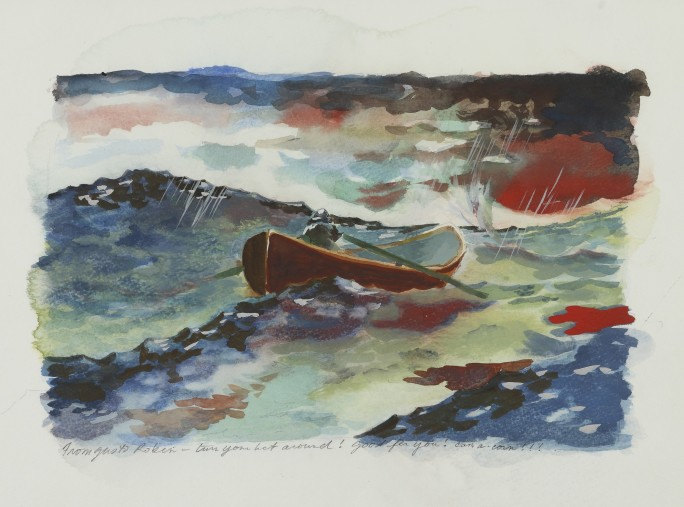
\includegraphics[width=0.75\textwidth]{boat_under_storm}
    \caption{Robin Williams's Prized Memento from \textit{Good Will Hunting} (1997).}
    \label{fig6}
\end{figure}
\textit{Have you ever noticed that there is the phrase ``logical'' at the tail end of the term ``psychological'', which seems to treat nonsense\texttt{/}non-logical arguments\texttt{/}events\texttt{/}situations from human bullshit after its logical counterpart seems so useless?} If anything is not logical\texttt{/}does not make sense in the 1st place, you should consider it with the psychological point of view instead, then perhaps it will be even more ``logical''\footnote{Like \textit{strong solutions} vs. \textit{generalized solutions} in the field of \href{https://en.wikipedia.org/wiki/Partial_differential_equation}{Partial Differential Equations} (PDEs).}.
 
\textit{At the end, what really matters for our life?}
\begin{quotation}
    Diane Nguyen: \textit{``It's too late. What's done is done.''}
    
    BoJack Horseman: \textit{``No.''}
    
    Diane Nguyen: \textit{``There's nothing I can do, BoJack. I'm not real. None of this is.''}
    
    BoJack Horseman: \textit{``So, what do I do now?''}
    
    Diane Nguyen: \textit{``BoJack, it doesn't matter.''}
    
    BoJack Horseman: \textit{``Well, if it doesn't matter, can I stay on the phone with you at least?''}
    
    Diane Nguyen: \textit{``Okay.''}
    
    BoJack Horseman: \textit{``How was your day?''}
    
    Diane Nguyen: \textit{``Good.''}
    
    BoJack Horseman: \textit{``Yeah?''}
    
    Diane Nguyen: \textit{``Yeah. My day was good.''} - BoJack Horseman vs. Diane Nguyen,  Episode: \textit{The View from Halfway Down}, \textit{BoJack Horseman} (2014--2020)
\end{quotation}
Watch e.g., \href{https://www.youtube.com/watch?v=Pt21dU5Pu8g}{BoJack Horseman - The View from Halfway Down}.\hfill$\square$

\begin{figure}[H]
    \centering
    \subfloat[\centering WTF did I just read?]{{
\includegraphics[height=8cm]{WTF_did_I_just_read}}}
    \qquad
    \subfloat[\centering Dafuq did I just write?]{{
\includegraphics[height=8cm]{dafug_I_just_read}}}
\end{figure}

\begin{verbatim}
    // ************************************************************************* //
\end{verbatim}

\begin{flushright}
    \textsc{Berlin, Germany}. Jan 2021.
    
    This text is a part of my \textit{personal project}: 
    
    \texttt{\#Series}: \textsc{Lost in Germany}.
\end{flushright}

%------------------------------------------------------------------------------%

\begin{thebibliography}{99}
    \bibitem[APA2013]{APA2013} American Psychiatric Association. \textit{\href{https://archive.org/details/diagnosticstatis0005unse/page/189}{Diagnostic and Statistical Manual of Mental Disorders (5th ed.)}}. Arlington: American Psychiatric Publishing. 2013. pp. 189--195. \textsc{isbn} 978-0890425558.
    
    \bibitem[Bancroft2003]{Bancroft2003} Bancroft, Lundy (2003). \href{https://www.amazon.com/Why-Does-He-That-Controlling/dp/0425191656}{\textit{Why Does He Do That?: Inside the Minds of Angry and Controlling Men}}. New York: Putnam's Sons, pp. 432. \textsc{isbn-10}: 0425191656. \textsc{isbn-13}: 978-0425191651
    
    \bibitem[Braiker2004]{Braiker2004} Braiker, Harriet B. (2004). \href{https://www.amazon.com/Whos-Pulling-Your-Strings-Manipulation/dp/0071446729}{\textit{Who's Pulling Your Strings?: How to Break the Cycle of Manipulation and Regain Control of Your Life}}. McGraw-Hill; 1st edition, pp. 256.  \textsc{isbn-10}: 0071446729. \textsc{isbn-13}: 978-0071446723.
    
    \bibitem[Dutton1994]{Dutton1994} Dutton, Donald G. (1994). ``Patriarchy and wife assault: the ecological fallacy''. Violence \& Victims. 9 (2): 167–182. \textsc{doi}: \href{https://doi.org/10.1891%2F0886-6708.9.2.167}{10.1891/0886-6708.9.2.167}. PMID 7696196. S2CID 35155731
    
    \bibitem[Dutton et al. 2000]{Dutton_Goodman_Bennett2000} Dutton, Mary Ann; Goodman, Lisa A.; Bennett, Lauren (2000). ``Court-involved battered women's responses to violence: the role of psychological, physical, and sexual abuse''. In Maiuro, Roland D.; O'Leary, K. Daniel (eds.), \textit{Psychological abuse in violent domestic relations}, New York: Springer Publishing Company, p. 197, ISBN 9780826111463.
    
    \bibitem[Kaplan and Thompson 1996]{Thompson_Kaplan1996}  Thompson, Anne E.; Kaplan, Carole A. (1996). ``Childhood emotional abuse''. \textit{The British Journal of Psychiatry}. 168 (2): 143--148. \textsc{doi}: \href{https://doi.org/10.1192%2Fbjp.168.2.143}{10.1192/bjp.168.2.143}. PMID 8837902
    
    \bibitem[FP2020]{FundamentalPessimist2020} \texttt{FundamentalPessimist} (2020). ``\href{https://www.reddit.com/r/AskAcademia/comments/fyffwg/i_want_to_out_my_toxic_phd_supervisor_on_social/}{I want to out my toxic PhD supervisor on social media (Twitter, LinkedIn, etc). What are the possible (legal) implications?}''. Reddit.
    
    \bibitem[NASEM2020]{NASEM2020} National Academies of Sciences, Engineering, and Medicine. 2020. \textit{Social Isolation and Loneliness in Older Adults: Opportunities for the Health Care System}. Washington, DC: The National Academies Press. \href{https://www.nap.edu/catalog/25663/social-isolation-and-loneliness-in-older-adults-opportunities-for-the}{https://doi.org/10.17226/25663}.
    
    \bibitem[Như Trang2020]{NhuTrang2020} Như Trang (2020). ``\href{https://trangtamly.blog/2020/04/07/goc-nhin-day-du-ve-co-lap-xa-hoi-social-isolation/}{Góc nhìn đầy đủ về Cô lập xã hội (Social Isolation)}''.
    
    \bibitem[\texttt{phill}2018]{phill2018} \texttt{phill} (2018). ``\href{https://academia.stackexchange.com/questions/111022/bad-relationship-with-phd-supervisor}{Bad relationship with PhD supervisor}''. Academia StackExchange.
    
    \bibitem[PsyWiki\texttt{/}AR]{Psychology Wiki/Abusive relationship} Psychological Wiki. ``\href{https://psychology.wikia.org/wiki/Abusive_relationship}{Abusive relationship}''.
    
    \bibitem[PsyWiki\texttt{/}PM]{Psychological Wiki/Psychological manipulation} Psychological Wiki. ``\href{https://psychology.wikia.org/wiki/Psychological_manipulation}{Psychological manipulation}''.
    
    \bibitem[Solomon2015]{Solomon2015} Solomon, Andrew (2015). \textit{The Noonday Demon}. 1st edition, pp. 688. \textsc{isbn-10}: 1501123882. \textsc{isbn-13}: 978-1501123887.
    
    \bibitem[Wiki\texttt{/}Anxiety disorder]{Wikipedia/Anxiety disorder} Wikipedia. ``\href{https://en.wikipedia.org/wiki/Anxiety_disorder}{Anxiety disorder}''.
    
    \bibitem[Wiki\texttt{/}BP]{Wikepedia/Breaking point (psychology)} Wikipedia. ``\href{https://en.wikipedia.org/wiki/Breaking_point_(psychology)}{Breaking point (psychology)}''.
    
    \bibitem[Wiki\texttt{/}D]{Wikipedia/Depression (mood)} Wikipedia. ``\href{https://en.wikipedia.org/wiki/Depression_(mood)}{Depression (mood)}''.
    
    \bibitem[Wiki\texttt{/}PA]{Wikipedia/Psychological abuse} Wikipedia. ``\href{https://en.wikipedia.org/wiki/Psychological_abuse}{Psychological abuse}''.
    
    \bibitem[Wiki\texttt{/}PM]{Wikipedia/Pyschological manipulation} Wikipedia. ``\href{https://en.wikipedia.org/wiki/Psychological_manipulation}{Psychological manipulation}''.
    
    \bibitem[Wiki\texttt{/}SI]{Wikipedia/Social isolation} Wikipedia. ``\href{https://en.wikipedia.org/wiki/Social_isolation}{Social isolation}''.
    
    \bibitem[Young-Powell2018]{Young-Powell2018} Young-Powell, Abby (2018). ``\href{https://www.theguardian.com/education/2018/jan/22/when-the-relationship-with-your-phd-supervisor-turns-toxic#comment-111169208}{When the relationship with your PhD supervisor turns toxic}''. \textit{The Guardian}.
\end{thebibliography}

\end{document}